% =====================================================================
% Chapter 4 — Experiments
% Drop-in for Overleaf. Required preamble (add to main.tex if missing):
%   \usepackage{booktabs}
%   \usepackage{graphicx}
%   \usepackage{subcaption}
%   \usepackage{xcolor}
%   \usepackage{multirow}
%   \usepackage{tcolorbox}      % for the illustrative case box
%   \usepackage{array}
%   \newcommand{\TBD}[1][--]{\textcolor{gray}{\textit{#1}}}
% Images expected next to main.tex (or in ./figs/):
%   overall_score.png   failure_modes.png
% =====================================================================

\section{Experiments}
\label{sec:experiments}

\subsection{Experimental Setup}
%已重写润色

\label{sec:exp-setup}



We evaluate 9 representative models on StartupBench, spanning both closed- and open-source families:
\begin{itemize}
    \item  \textbf{Closed-source}:  GPT-5.6-sol~\cite{openai2026gpt56}, GPT-5.5 ~\cite{openai_gpt55}, Gemini-3.1-Pro~\cite{GoogleCloud2026Gemini3.1Pro}, Seed-2.1-Pro~\cite{bytedance2026seed21},Qwen-3.6-Max~\cite{qwen36_max_preview}

    \item \textbf{Open-source}: DeepSeek-V4-Pro~\cite{deepseek2026v4},Kimi-K3 \cite{team2026kimi}, Kimi-K2.6~\cite{moonshot2026k2_6},  GLM-5.1~\cite{zeng2026glm}.
\end{itemize}
To improve the reliability of our results, we conduct \textbf{3} independent runs for each model and report 95\% bootstrap confidence intervals for the task scores, computed using 10{,}000 resamples.
All models are executed under the same Nanobot harness with an identical tool configuration, and every task is capped at a maximum of \textbf{200} interaction steps.
For each task, the agent is initialized with the task-specific workspace and input query, and its deliverables are collected from the designated output directory. Following the evaluation protocol described in the previous section, the deliverables are evaluated by the judge agent against the task specification, workspace context, and rubric set.

For automatic evaluation, the judge agent also runs under the same Nanobot harness to ensure a consistent execution environment, while using GPT-5.5 as the underlying judge model. Apart from the continuous task score, we also report \textbf{success rate}, the fraction of runs that are successfully completed, pooled over the three runs. A task is considered successful if its final score is at least \textbf{90}; otherwise, it is counted as a failure.



\subsection{Main Results}
%已重写润色
\label{sec:exp-overall}

\begin{figure}[t]
%leaderboard需要更新分数后重画。
  \centering
  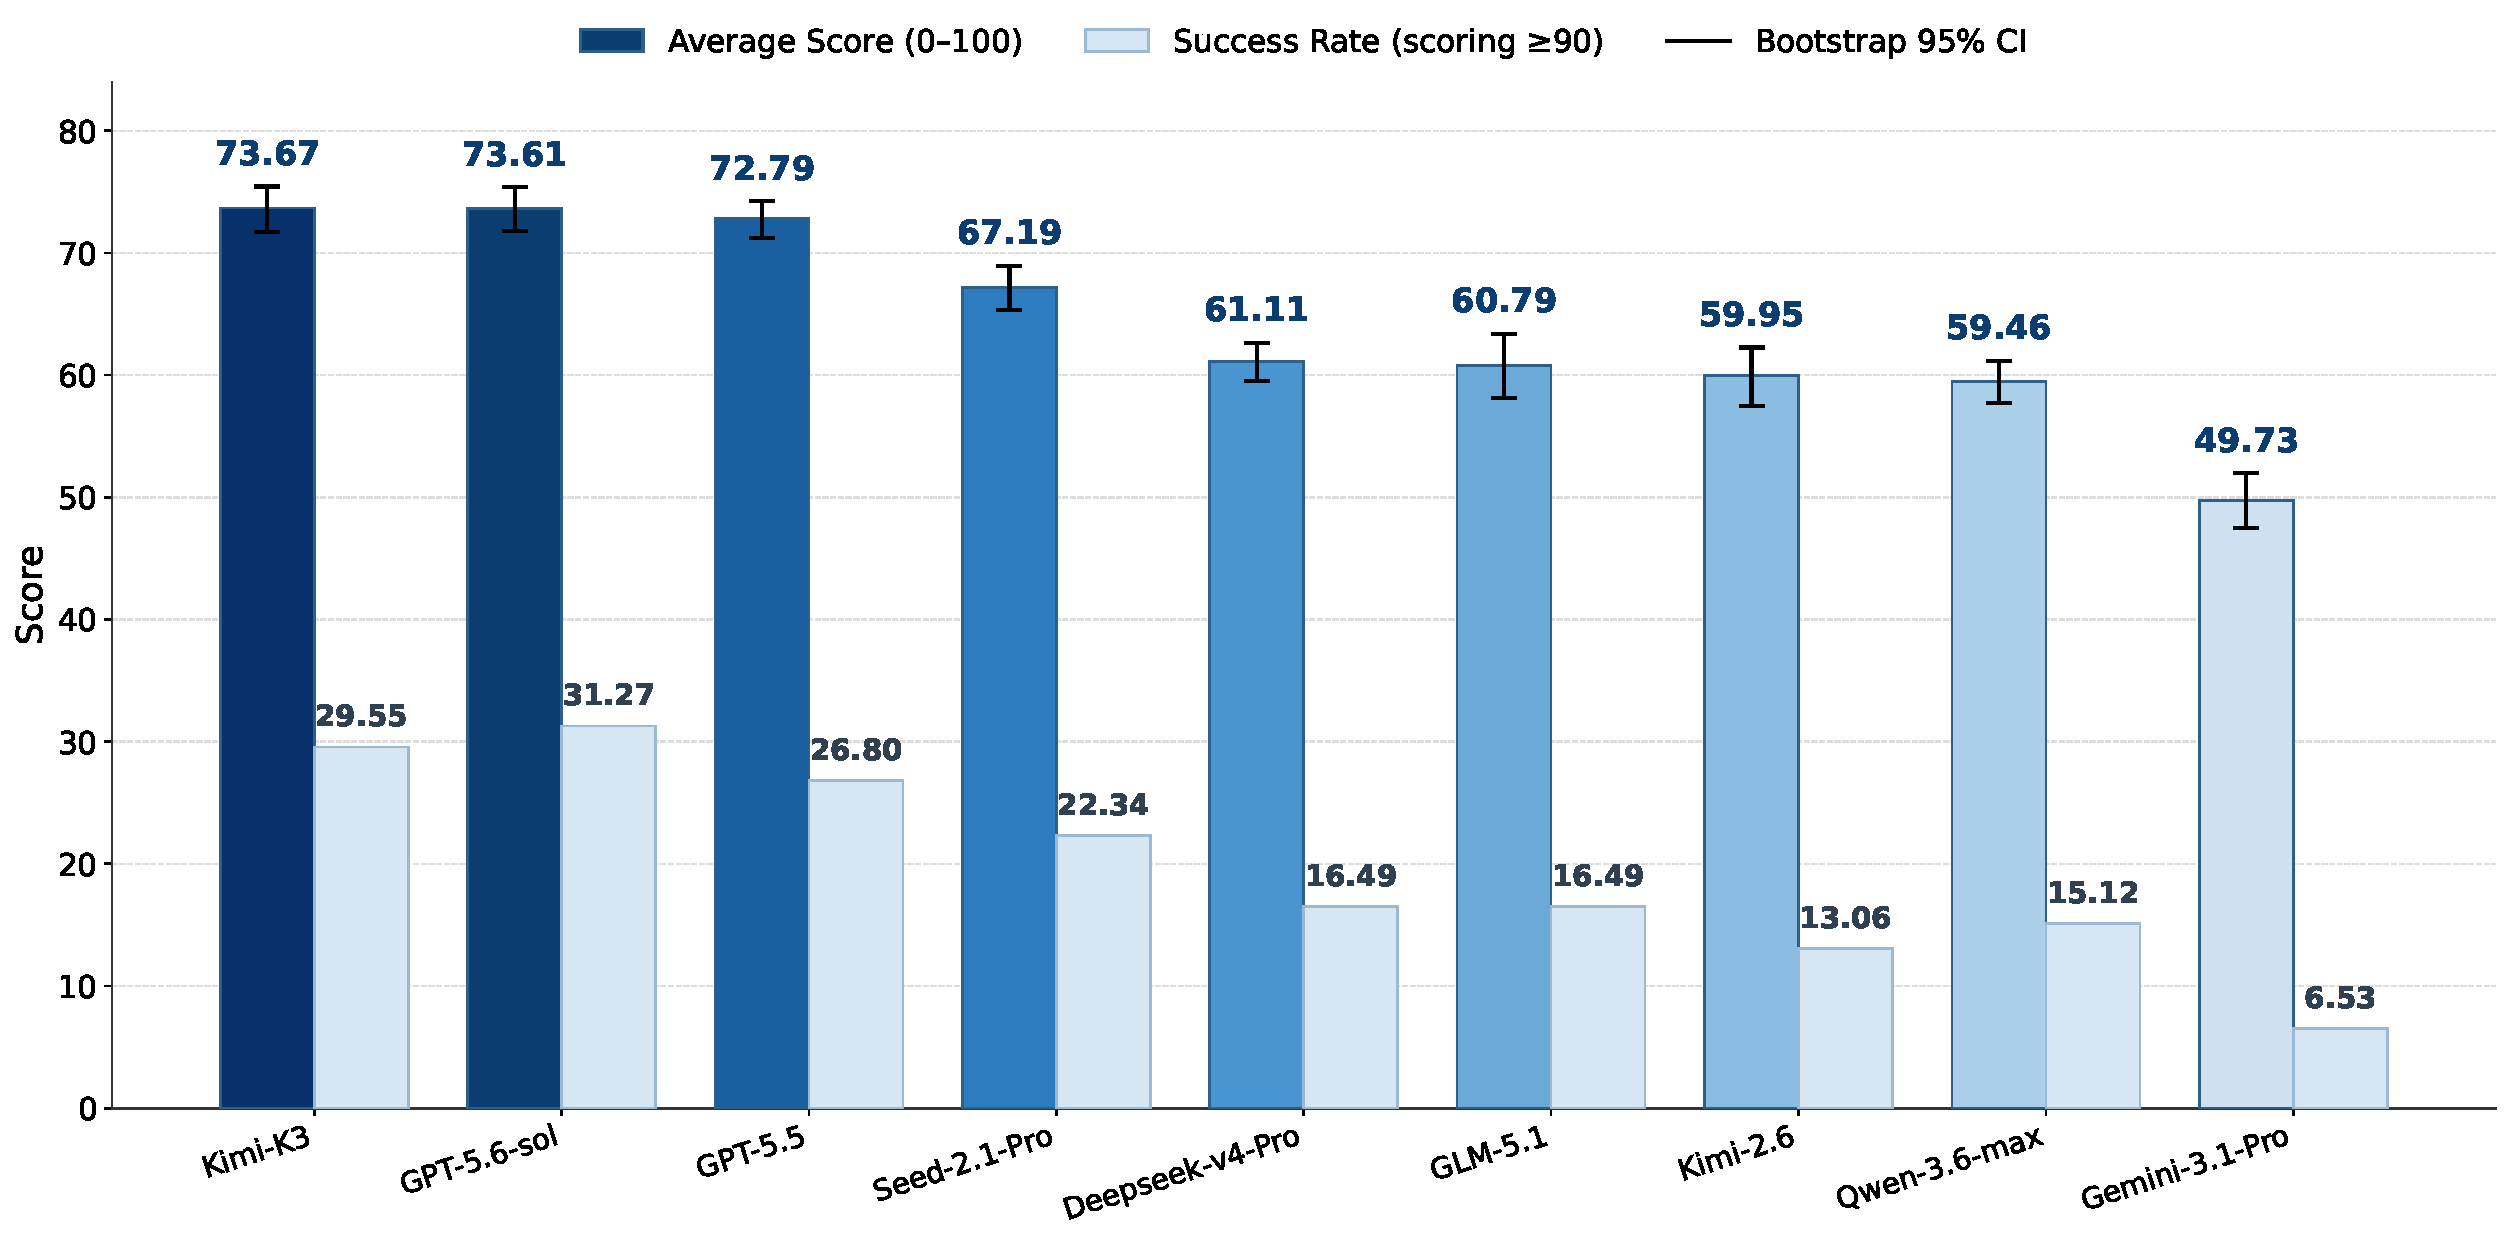
\includegraphics[width=0.95\linewidth]{figures/overall_score_bs_out.pdf}
  \caption{Leaderboard of StartupBench.}
  \label{fig:overall-leaderboard}
\end{figure}
% TODO:竖着/增加pass1/颜色 done

\begin{table*}[t]
  \centering
  \small
  \setlength{\tabcolsep}{5pt}
  \renewcommand{\arraystretch}{1.15}
  \caption{Model performance of StartupBench, averaged over three independent runs.
    \textbf{Top block:} importance-weighted mean per-task score ($0$--$100$);
    \textbf{bottom block:} success rate, the fraction of samples scoring $\ge 90$ (\%),
    pooled over the three runs. Per-column \textbf{best in bold},
    \underline{second-best underlined}.}
  \label{tab:leaderboard}
  \begin{tabular}{lccccccc}
    \toprule
    \textbf{Model} & \textbf{Overall}
      & \textbf{Med} & \textbf{Finance} & \textbf{Legal}
      & \textbf{Business} & \textbf{STEM} & \textbf{Education} \\

    \midrule
    \multicolumn{8}{c}{\textbf{Average score}} \\
    \midrule
    Kimi-K3 & \textbf{73.67} & \textbf{80.03} & \textbf{62.38} & 69.45 & \textbf{83.90} & 68.34 & \textbf{77.71} \\

    GPT-5.6-sol & \underline{73.61} & \underline{79.32} & 61.66 & \textbf{73.53} & 77.61 & \textbf{74.77} & \underline{73.94} \\

    GPT-5.5         & 72.79 & 78.59 & \underline{62.09} & \underline{71.75} & \underline{79.59} & \underline{72.14} & 68.32 \\
    Seed-2.1-Pro    & 67.19 & 73.15 & 57.26 & 61.35 & 77.83 & 65.61 & 62.91 \\
    Kimi-K2.6       & 59.95 & 67.70 & 51.17 & 54.62 & 71.91 & 51.38 & 58.60 \\
    GLM-5.1         & 60.79 & 65.66 & 51.22 & 50.20 & 78.53 & 52.18 & 66.50 \\
    Qwen-3.6-Max    & 59.46 & 66.51 & 52.45 & 50.33 & 75.03 & 48.83 & 59.26 \\
    DeepSeek-V4-Pro & 61.11 & 69.42 & 51.11 & 54.53 & 73.69 & 54.89 & 57.03 \\
    Gemini-3.1-Pro  & 49.73 & 54.05 & 41.00 & 43.49 & 61.18 & 45.88 & 51.23 \\
    \midrule
    \multicolumn{8}{c}{\textbf{Success rate}\, ($\ge90$)} \\
    \midrule
    Kimi-K3 & \underline{29.55} & \textbf{34.92} & 20.37 & 20.83 & \textbf{52.63} & 16.67 & \underline{23.81} \\
    GPT-5.6-sol & \textbf{31.27} & \underline{33.33} & \textbf{27.78} & \underline{22.92} & 38.60 & \textbf{33.33} & \textbf{28.57} \\

    GPT-5.5         & 26.80 & 30.16 & \underline{22.22} & \textbf{25.00} & 38.60 & \underline{22.92} & 9.52 \\
    Seed-2.1-Pro    & 22.34 & 19.05 & 16.67 & 14.58 & \underline{45.61} & 20.83 & 4.76 \\
    Kimi-K2.6       & 13.06 & 15.87 & 14.81 & 6.25 & 24.56 & 4.17 & 4.76 \\
    GLM-5.1         & 16.49 & 12.70 & 16.67 & 8.33 & 36.84 & 8.33 & 9.52 \\
    Qwen-3.6-Max    & 15.12 & 11.11 & 16.67 & 10.42 & 33.33 & 6.25 & 4.76 \\
    DeepSeek-V4-Pro & 16.49 & 20.63 & 16.67 & 8.33 & 29.82 & 10.42 & 0.00 \\
    Gemini-3.1-Pro  & 6.53 & 6.35 & 11.11 & 6.25 & 8.77 & 0.00 & 4.76 \\
    \bottomrule
  \end{tabular}
\end{table*}

\textbf{Startup tasks remain far from saturated under a general-purpose agent harness.} Although the strongest models, Kimi-K3 and GPT-5.6-sol, achieve average scores of 73.67\% and 73.61\%, respectively, no model successfully completes even one third of the benchmark under the strict acceptance criterion (score $\ge 90$). More broadly, the average scores of most models lie between roughly 55 and 75, indicating that current agents are generally capable of making substantial progress toward solving realistic professional workflows. However, high average scores do not necessarily translate into high task completion rates. This is particularly evident for the Kimi series: Kimi-K3 achieves the highest average score overall but a lower success rate than GPT-5.6-sol, while Kimi-K2.6 similarly attains a higher average score than Qwen-3.6-Max but a lower success rate. These discrepancies suggest that some models can satisfy a substantial fraction of task requirements while still falling short of complete delivery. More generally, all models exhibit substantially lower success rate than average score, suggesting that the primary bottleneck is no longer executing large portions of a workflow, but consistently producing artifacts that satisfy the standards required for direct professional use.

This gap has two important implications. First, it helps explain why specialized vertical agents continue to provide practical value in many market-validated workflows, where consistently meeting professional standards remains essential. Second, it suggests that the next frontier for foundation models is not merely performing professional tasks, but reliably producing work products that users can adopt without further verification or revision. We further investigate the underlying causes of this gap in Section~\ref{sec:exp-failures}.


\textbf{Performance varies substantially across professional domains.} Table 3 reveals that current general-purpose agents do not exhibit uniform competence across real-world workflows. Among the six domains, Business is consistently the easiest: every model achieves an average score above 60, and the average success rate across models is also substantially higher than in any other domain. In contrast, Finance is the most challenging, with the lowest average score of 54.48\%. The large gap between Business and Finance suggests that current models handle structured, relatively standardized tasks more reliably than workflows requiring sustained quantitative reasoning, cross-document consistency, and multi-step verification.

The results also reveal pronounced domain specialization. While Kimi-K3 and GPT-5.6-sol achieve nearly identical average scores overall (73.67 vs. 73.61), their strengths differ substantially across domains. Under success rate, Kimi-K3 performs best in Medical and Business, whereas GPT-5.6-sol leads in Finance, STEM, and Education; GPT-5.5 remains strongest in Legal. A similar pattern emerges in average score, where Kimi-K3 leads in Medical, Business, Finance and Education, GPT-5.6-sol in Legal and STEM. Thus, even among the strongest models, no single agent consistently dominates across professional domains. These results suggest that current general-purpose agents still exhibit substantial domain-dependent variation, leaving considerable room for improving the robustness and transferability of end-to-end task execution across heterogeneous professional workflows.


% \paragraph{Reliability of the grouping.}
% The three-group reading survives the two checks that could undermine it:
% a finite task pool and an automatic judge. The task-level Bootstrap
% yields overall-mean CI half-widths of $\pm 5$ to $\pm 6$ points, so
% differences below roughly $10$ points are within sampling noise; this
% is enough to separate the leading, middle, and trailing groups while
% leaving the order within each group statistically indistinct, which is
% why we describe groups rather than a strict ranking. The automatic
% judge is validated against expert re-grading (\S\ref{sec:exp-agreement}),
% which agrees with it on over $91\%$ of rubric verdicts. The grouping is
% thus robust both to resampling the task pool and to substituting human
% experts for the judge.

\subsection{Effectiveness of Proposed Evaluation Framework}
%已重写润色
\label{sec:exp-agreement}

%暂时勿动





To validate the reliability of our evaluation framework, we compare its judgments against expert annotations. We sample outputs from two representative models for all tasks and ask domain experts to independently evaluate each submission using the predefined rubrics. At the rubric level, the automatic evaluator achieves an overall agreement of \textbf{92.78\%} with expert judgments. We further examine whether these local agreements translate into consistent task-level decisions by comparing the resulting success labels, where a submission is considered successful if its aggregated score reaches 90. The automatic and expert evaluations agree on \textbf{92.84\%} of these success decisions. Notably, the similarly high agreement at both rubric and success levels, despite their substantially different label distributions, suggests that the observed consistency is not merely an artifact of label imbalance.


We further investigate the necessity of evaluating each rubric independently. As an ablation, instead of assigning one rubric to one judge agent, we directly provide the complete model output together with the full rubric list to a single judge agent, requiring it to score all rubrics in one end-to-end inference. This alternative reduces the agreement with human experts to \textit{83\%}. More importantly, the holistic setting proves considerably less stable in practice. Since the judge agent must simultaneously perform long-context reasoning, maintain consistency across numerous evaluation criteria, and finally generate a structured output covering all rubric scores, failures such as malformed outputs or incomplete formatting frequently occur, forcing repeated executions. On average, each evaluation requires more than two runs before a valid result is obtained. In contrast, our rubric-wise evaluation decomposes the assessment into a collection of independent, lightweight judging tasks, yielding both substantially higher agreement with human experts and significantly better execution robustness.




\subsection{Failure-Mode Analysis}
%需要大幅度重写润色，理想状态是统计分析和case study结合。目前缺以下统计：不同类型rubric模型表现统计，大/复杂输入文件系统题目的模型表现，文件格式问题rubric统计。

\subsubsection{Outcome-level Failure Analysis}
\label{sec:exp-format}

\begin{figure*}[t]
    \centering
    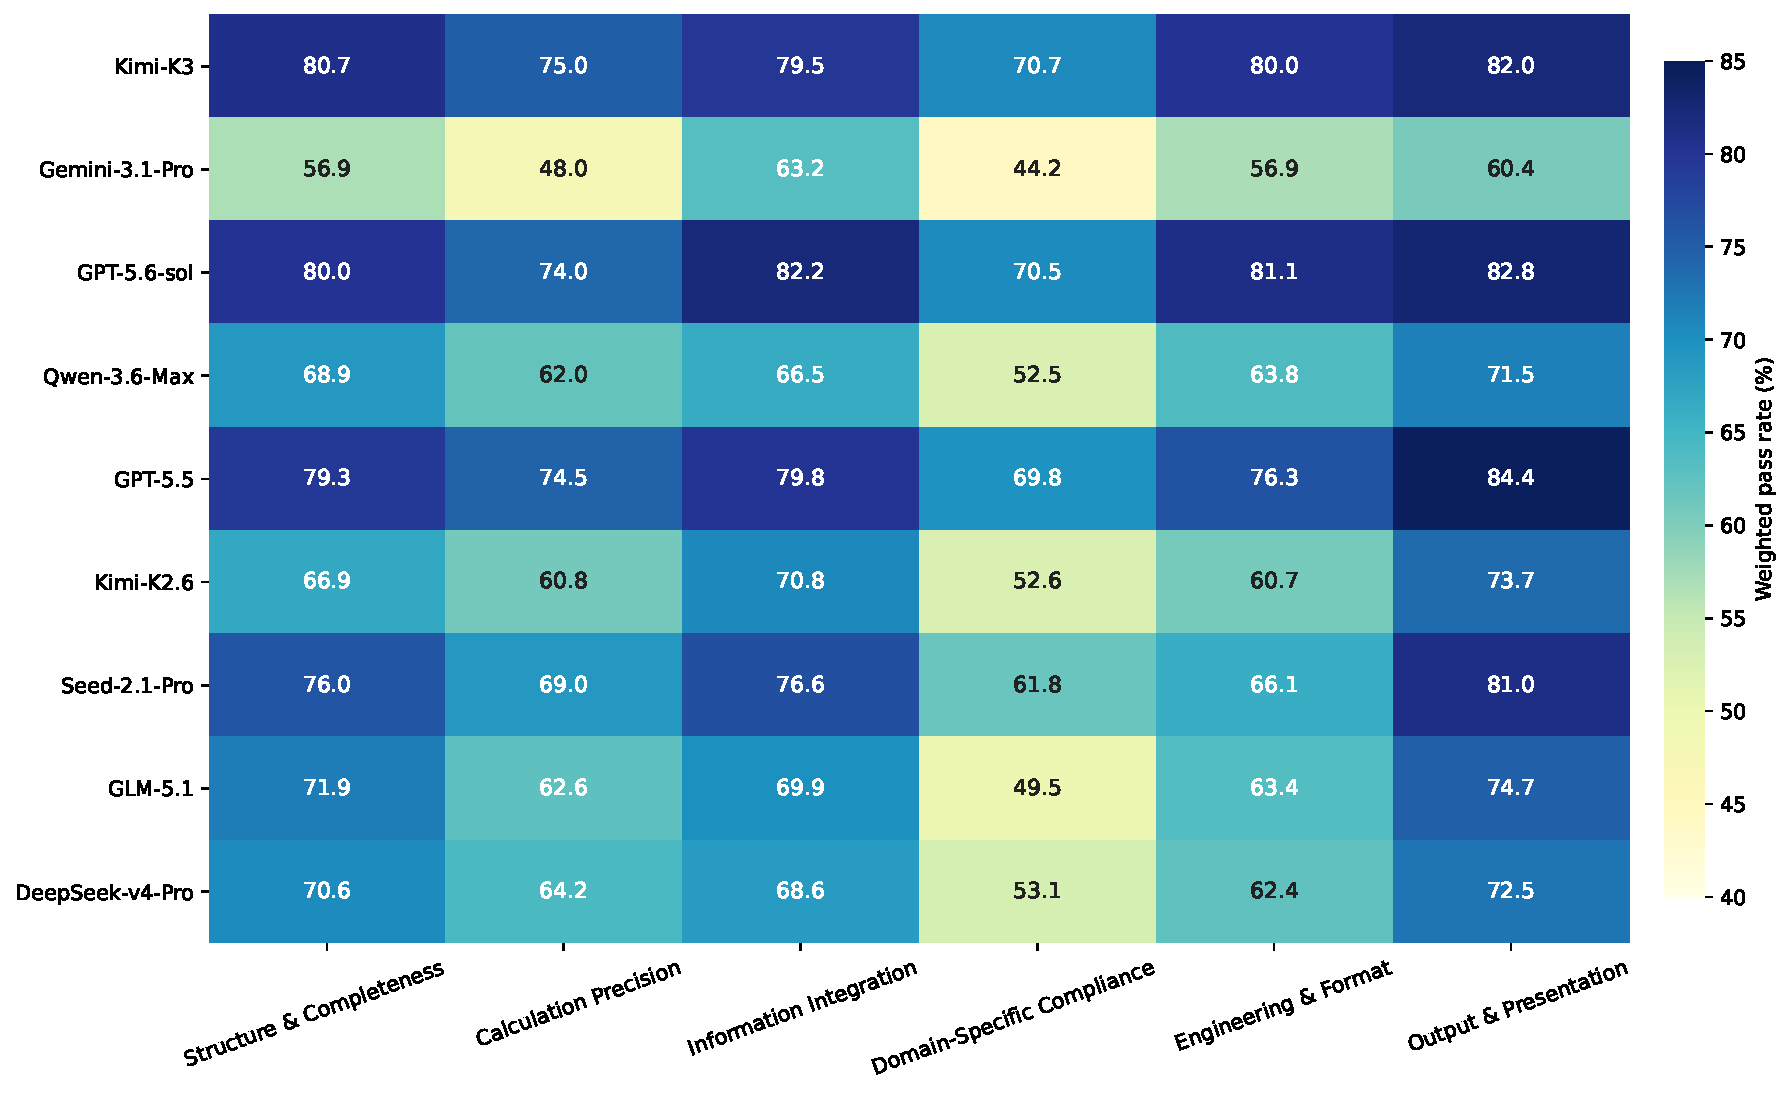
\includegraphics[width=0.99\textwidth]{figures/heatmap_9model.pdf}
    \caption{
Performance across rubric dimensions. Importance-weighted pass rates (\%) of different models on the six rubric dimensions in StartupBench. Higher values indicate better performance under the corresponding evaluation dimension.
    }
    \label{fig:dimension-rubric}
% \vspace{-6pt}
\end{figure*}


\textbf{Capability differences across rubric dimensions.} Figure~\ref{fig:dimension-rubric} further breaks down model performance by rubric dimension. Overall, current models achieve consistently higher scores on Structure \& Completeness, Information Integration, and especially Output \& Presentation, indicating that they are generally capable of organizing heterogeneous information into well-structured and visually polished deliverables. In contrast, Domain-Specific Compliance emerges as the most challenging dimension across all evaluated models, while Calculation Precision also remains substantially weaker than the other dimensions. This suggests that although modern foundation models can produce artifacts that appear complete and professional, reliably satisfying domain-specific regulations, business conventions, and numerical correctness continues to be a major obstacle for real-world deployment.

The two strongest models, GPT-5.6-sol and Kimi-K3, outperform the remaining systems across nearly all rubric dimensions rather than relying on a single specialized capability. Their largest advantages are observed in Structure \& Completeness, Calculation Precision, Information Integration, and Output \& Presentation, demonstrating stronger end-to-end workflow execution and artifact construction capabilities. Nevertheless, even these leading models obtain their lowest scores on Domain-Specific Compliance, indicating that adherence to professional standards and domain-specific requirements remains the primary bottleneck even for state-of-the-art systems.



\textbf{Models often satisfy peripheral requirements while missing what matters most.}
Table~\ref{tab:corefail} reports task-normalized rubric satisfaction rates across the three importance levels. Averaged across models, satisfaction decreases from \textbf{68.67\%} for Auxiliary rubrics to \textbf{65.89\%} for Important rubrics and \textbf{63.45\%} for Core rubrics, with 8 of the 9 models exhibiting the same overall trend. Importantly, these levels reflect each requirement's contribution to successful task completion rather than its expected difficulty. This pattern reveals a characteristic failure mode of current agents: they can often fulfill auxiliary or surface-level requirements while failing on the core requirements that determine whether the task is actually completed successfully. In other words, substantial apparent progress can be driven by satisfying less consequential parts of the task, while critical omissions still prevent the final deliverable from being practically usable.

A typical case of models struggling with requirements central to task completion is shown in Figure~\ref{fig:corefail}. In this mechanical process task, models often complete peripheral workbook requirements but fail on the core technical operations: extracting dimensions accurately from engineering drawings, validating specifications against the provided documents, and linking identified discrepancies to the corresponding rectification actions. These failures prevent the resulting workbook from fulfilling its primary purpose even when many auxiliary requirements are successfully completed.



\begin{table}[t]
\centering
\small
\caption{Task-normalized rubric satisfaction rates (\%) across different importance levels.
For each model--task--trial, we first compute the satisfaction rate within each importance level and then average across tasks and trials.}
\label{tab:corefail}
\begin{tabular}{lccc}
\toprule
\textbf{Model}
& \textbf{Auxiliary }
& \textbf{Important }
& \textbf{Core } \\
\midrule
Kimi-K3          & 77.89 & 75.12 & 73.40 \\
GPT-5.6-sol      & 77.59 & 74.47 & 73.07 \\
GPT-5.5          & 75.12 & 75.09 & 72.07 \\
Seed-2.1-Pro         & 70.83 & 69.85 & 65.77 \\
Kimi-K2.6        & 66.64 & 63.56 & 57.82 \\
GLM-5.1          & 64.58 & 61.40 & 60.68 \\
Qwen-3.6-Max     & 65.39 & 62.17 & 58.08 \\
DeepSeek-V4-Pro  & 66.50 & 62.97 & 60.05 \\
Gemini-3.1-Pro       & 53.48 & 48.41 & 50.13 \\
\midrule
\textbf{Average} & \textbf{68.67} & \textbf{65.89} & \textbf{63.45} \\
\bottomrule
\end{tabular}
\end{table}




\begin{figure*}[t]
    \centering
    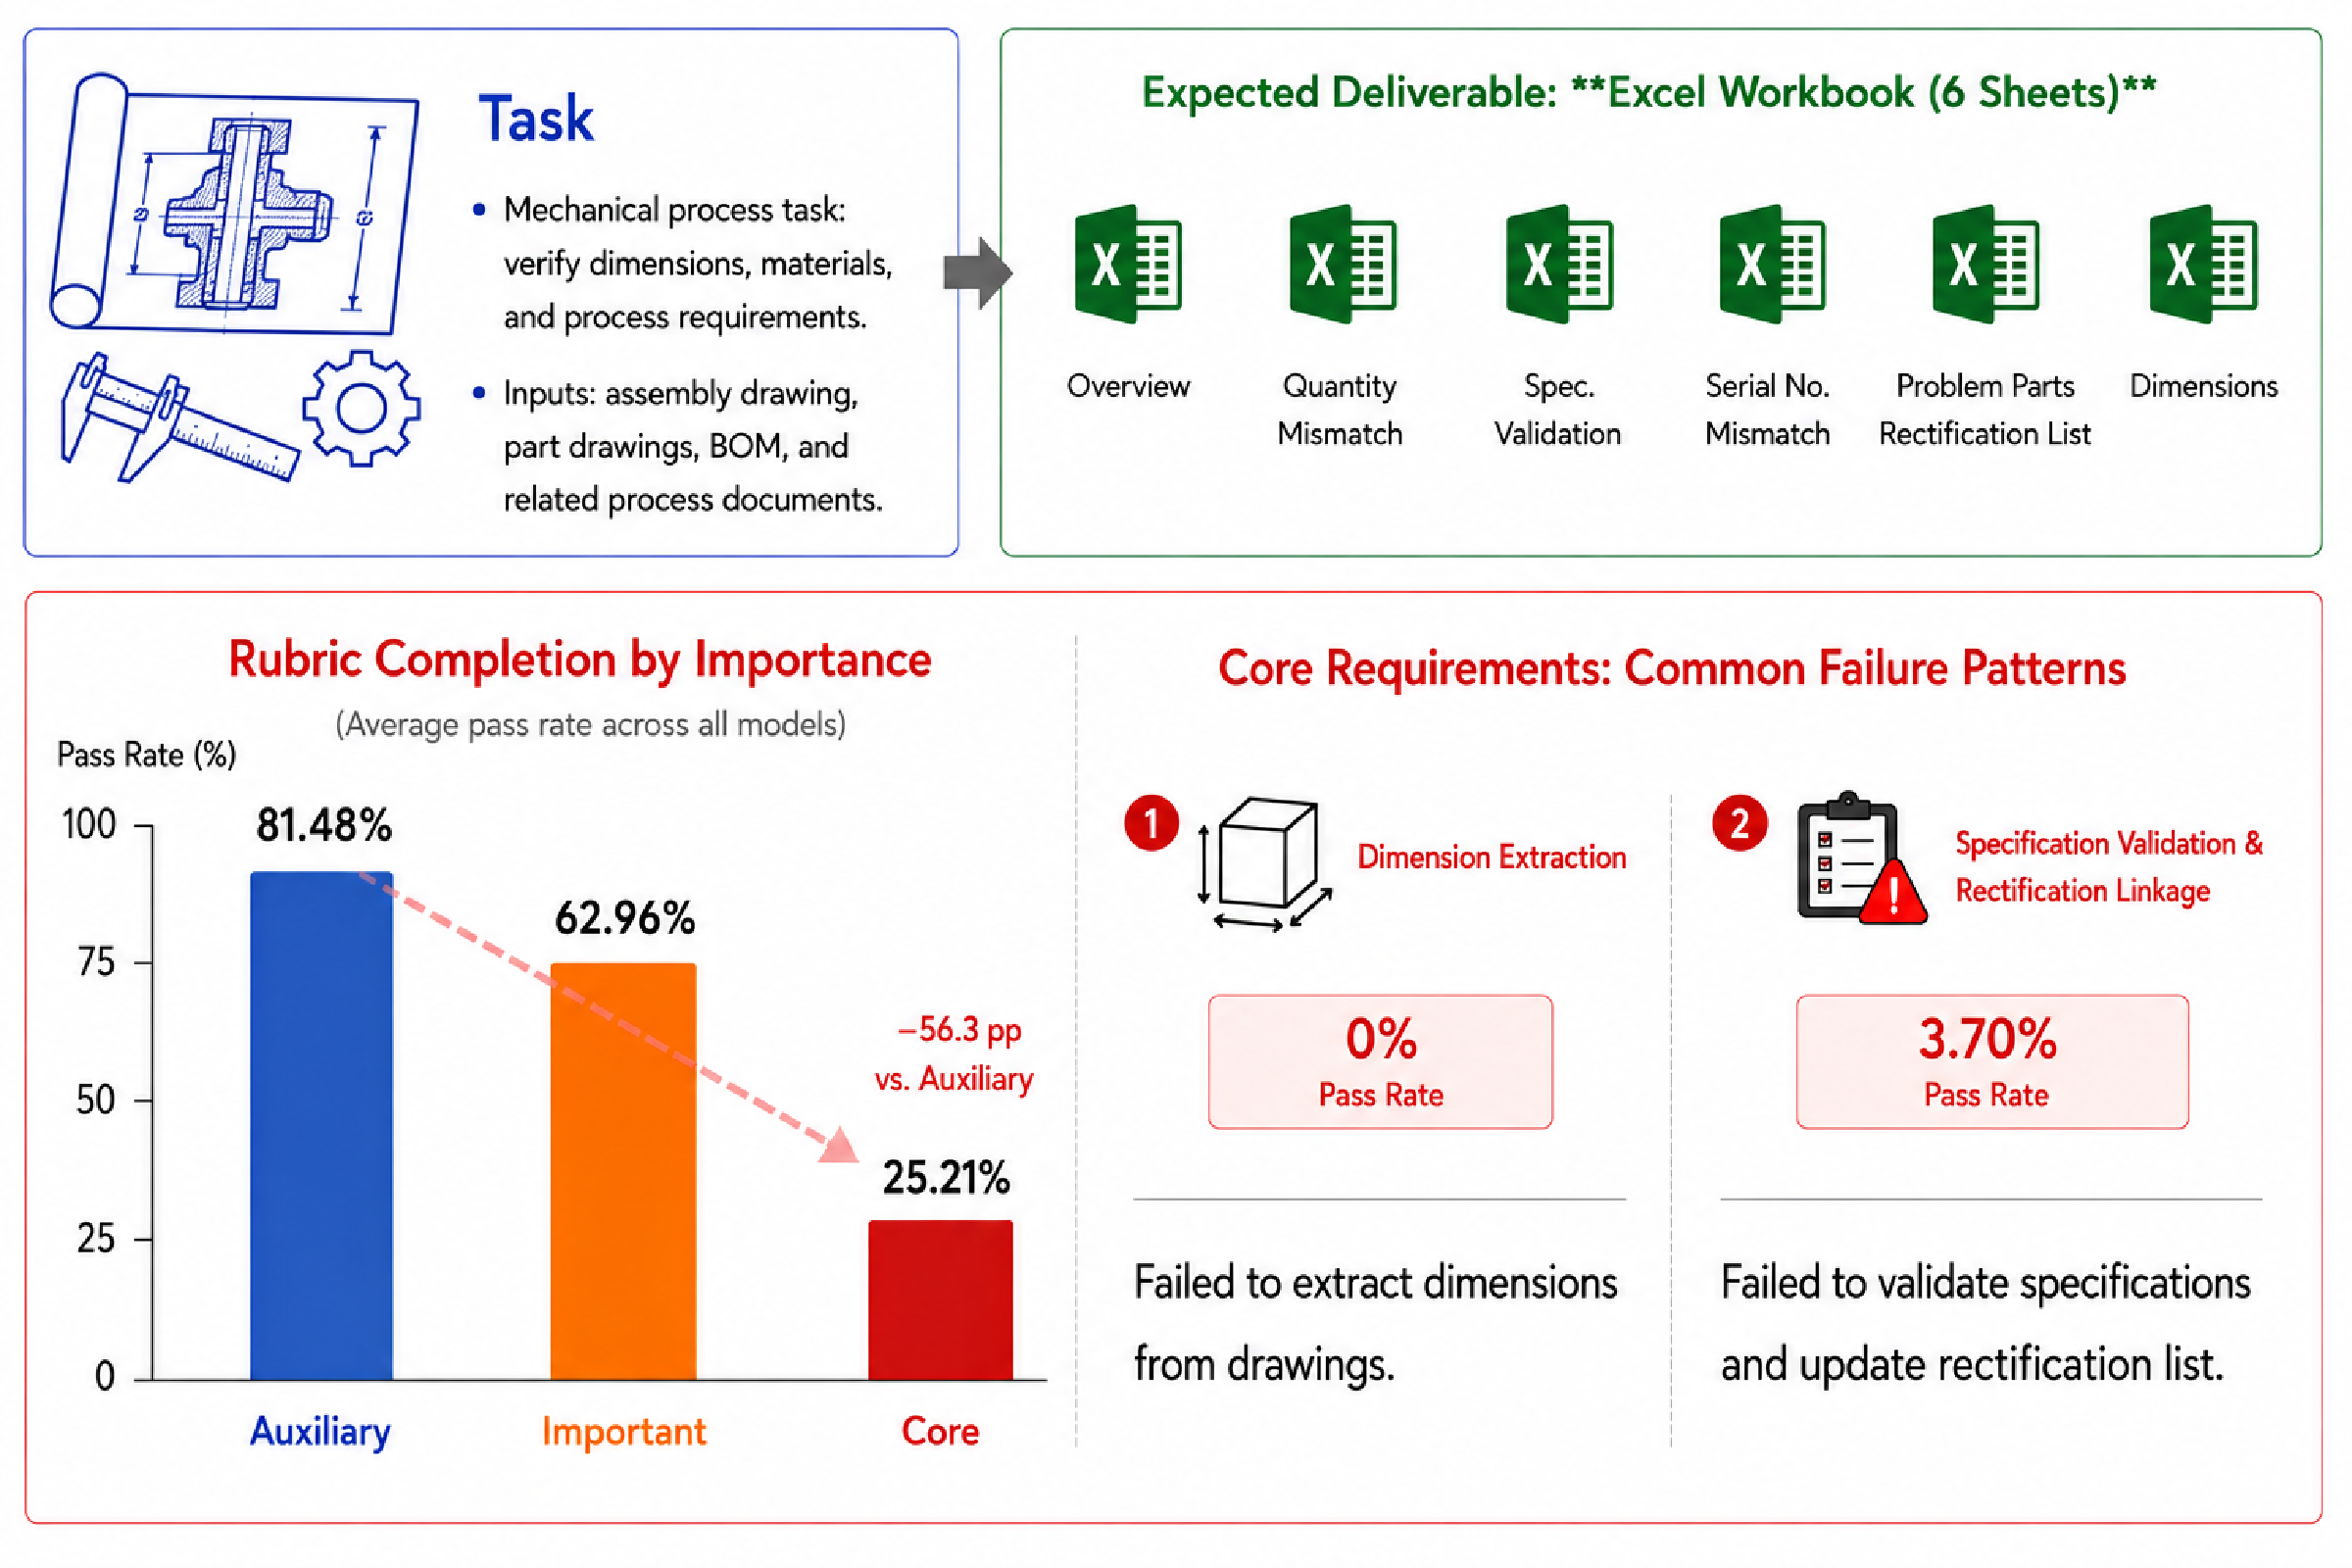
\includegraphics[width=0.8\textwidth]{figures/rubric_corefail_case.pdf} %图还需要改
    \caption{
A representative case of models failing on core rubrics though passing auxiliary rubrics on StartupBench.
    }
    \label{fig:corefail}
% \vspace{-6pt}
\end{figure*}



\textbf{Output format non-compliance.}
Some failures arise from models not producing deliverables in the file type explicitly required by the task. Unlike most failure modes discussed above, this requirement involves neither complex reasoning nor domain knowledge and can be verified deterministically from file extensions. Nevertheless, no model achieves perfect compliance on the 56 tasks with explicit output-format requirements (Table~\ref{tab:format-compliance}), with success rates ranging from $97.6\%$ to $86.3\%$. Most violations fall into two recurring patterns: generating an incorrect file type (e.g., returning \texttt{.md}/\texttt{.txt} instead of the required \texttt{.pdf}) and omitting part of the requested deliverables (e.g., producing only one of the required \texttt{.xlsx} and \texttt{.docx} files). These errors suggest that even elementary deliverable-level constraints remain a non-negligible source of failures for current foundation models.

\begin{table}[t]
\centering
\footnotesize
\caption{Output-format compliance on the 56 StartupBench tasks with explicit output-file requirement rubrics. Models are ranked by compliance rate.}
\label{tab:format-compliance}
\begin{tabular}{lc}
\toprule
\textbf{Model} & \textbf{Compliance (\%)}\\
\midrule
Kimi-K3           & 97.6 \\
Seed-2.1-Pro      & 95.2 \\
GPT-5.6-sol       & 94.6 \\
Qwen-3.6-Max      & 94.6 \\
DeepSeek-V4-Pro   & 94.0 \\
GPT-5.5           & 93.5 \\
Kimi-K2.6         & 92.9 \\
Gemini-3.1-Pro    & 86.9 \\
GLM-5.1           & 86.3 \\
\bottomrule
\end{tabular}
\end{table}


\subsubsection{Behavior-level Failure Analysis}
\label{sec:exp-failures}
\textbf{Complex Instruction Following.} Complex real-world workflows typically impose numerous constraints on the final deliverable, including structural organization, computation logic, formatting, and executable correctness. Although these requirements are explicitly specified in the task description, current models frequently exhibit partial compliance: they satisfy the most visible requirements while overlooking other equally critical constraints. As a result, the generated artifact appears largely complete from a superficial inspection, yet fails to satisfy the complete acceptance criteria required for direct use. This behavior indicates that models often optimize for producing outputs that look correct, rather than ensuring that every instruction governing the final deliverable has been faithfully executed.

A representative example is shown in Figure~\ref{fig:instruction}. The task requires generating a complete HR payroll workbook from multiple source sheets under a diverse set of structural, computational, and formatting constraints. Although the model produces an artifact that appears largely complete—including all required worksheets, formulas, charts, and dashboard layouts—the artifact-level evaluation reveals that several critical acceptance conditions remain unsatisfied. Specifically, key cached values required for downstream verification are missing, rendering the workbook unverifiable despite its polished appearance. This case illustrates a common pattern of partial compliance, where the model satisfies the most visible requirements while overlooking less obvious but equally essential deliverable constraints.

\begin{figure*}[t]
    \centering
    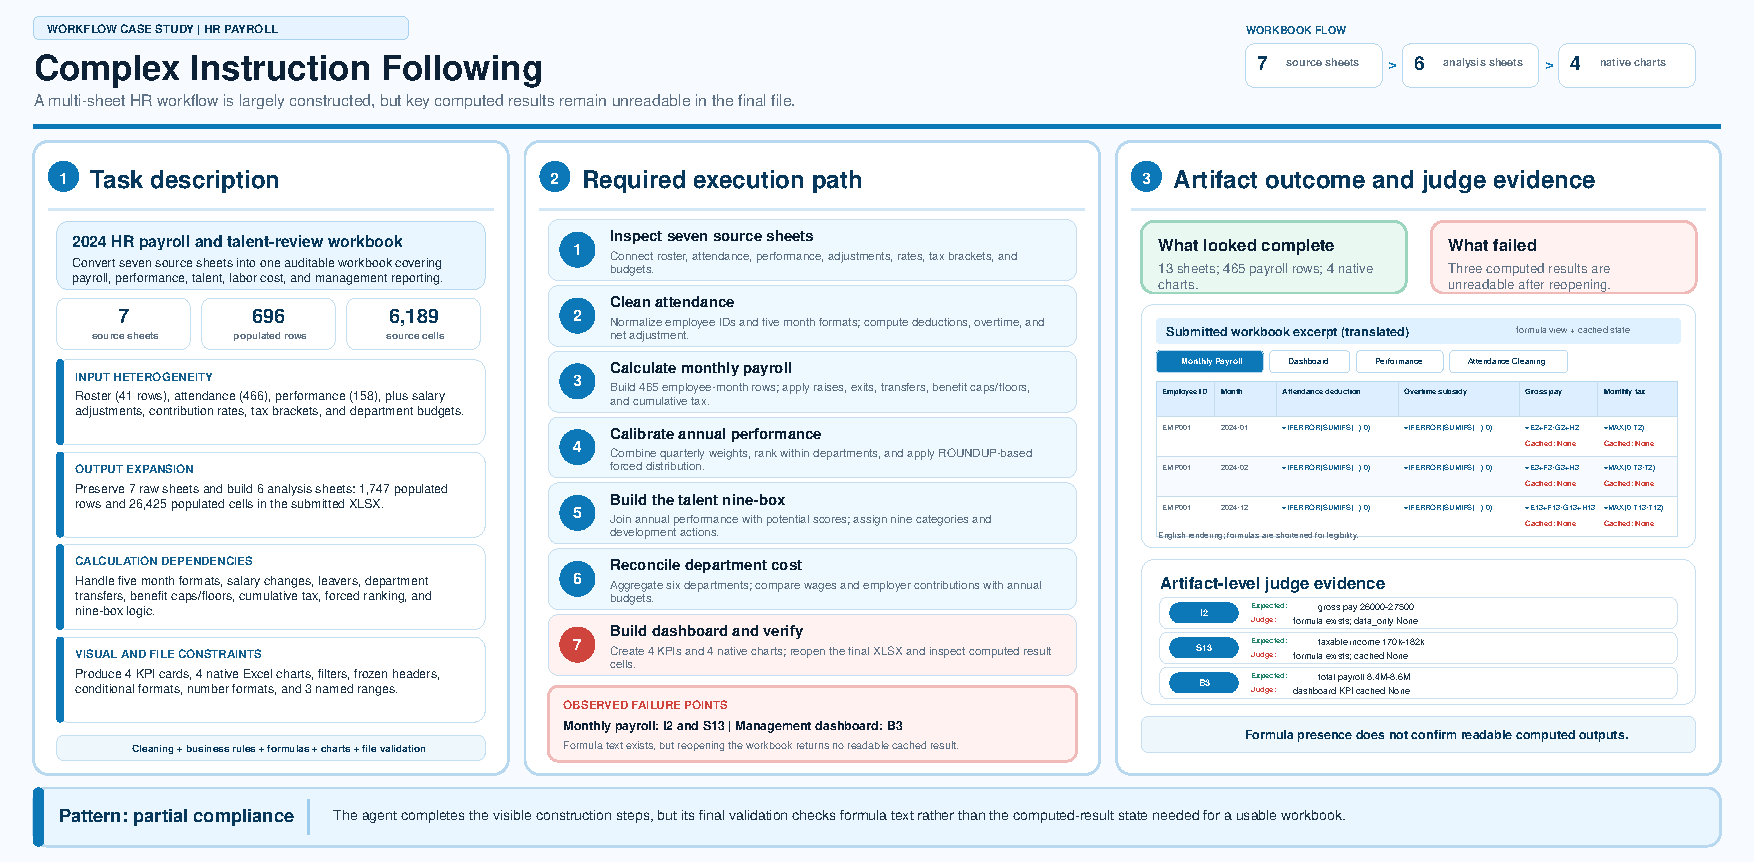
\includegraphics[width=0.99\textwidth]{figures/figure5_hr.pdf} %图还需要改
    \caption{
A representative case of complex instruction following failure.
Although the generated workbook appears complete, artifact-level evaluation reveals that several critical acceptance conditions remain unsatisfied, illustrating a common pattern of partial compliance.
    }
    \label{fig:instruction}
% \vspace{-6pt}
\end{figure*}


\textbf{Self-Verification Hallucination.} We also observe that many models fail not because they cannot complete the required workflow, but because they incorrectly assume that successful execution implies successful delivery. After producing a plausible artifact, the model often summarizes the intended reasoning process or completed steps as evidence that the task has been verified, without independently inspecting the final deliverable against the original user requirements. Consequently, subtle yet critical errors—such as incorrect cell values, unmatched identifiers, missing constraints, or formatting inconsistencies—remain undetected despite an otherwise convincing output. This behavior reflects a form of self-verification hallucination, where the model mistakes confidence in its own reasoning process for evidence that the generated artifact satisfies the acceptance criteria. In real-world office workflows, however, successful completion requires validating the final deliverable itself rather than merely confirming the execution process, making this a common source of deployment-critical failures. A typical case is shown at Appendix~\ref{app:self-verify hallucination}.


\textbf{Domain-Specific Expertise.} Another major source of failure arises from insufficient domain-specific expertise, consistent with the relatively poor performance on the Domain-Specific Compliance dimension. Unlike general instruction-following errors, these failures are driven by the unique operational requirements of different professional domains. Although models often generate outputs that appear fluent and professionally formatted, they frequently fail to satisfy the domain-specific constraints that determine whether a deliverable is actually usable. As a result, the dominant failure patterns vary substantially across domains, reflecting different notions of correctness, evidence, precision, and actionability required by real-world workflows.

From a domain perspective, different professional areas expose distinct failure characteristics. Business and management tasks primarily stress artifact correctness, particularly for spreadsheets, dashboards, formulas, and structured reports. Finance tasks emphasize source attribution, numerical precision, valuation assumptions, and temporal consistency, where errors commonly arise from insufficient reconciliation, inadequate numerical self-verification, or inconsistent accounting conventions. Legal tasks are less constrained by legal writing style than by the completeness and correctness of legal reasoning, including missing citations, incomplete factual coverage, insufficient statutory support, or incorrect mapping between facts and applicable rules. Medical tasks achieve relatively higher average scores but pose substantially greater safety risks, since mistakes in medication timing, continuation criteria, or discharge planning directly undermine clinical usability. STEM and Computer Science tasks instead require precise object-level grounding, demanding accurate relationships among code, engineering drawings, images, bills of materials, and system components. Finally, education and humanities tasks place greater emphasis on fine-grained rule following, such as curriculum requirements, credit allocation, document organization, and textual coherence. A typical example of failure caused by
insufficient domain-specific expertise is shown at Appendix~\ref{app:domain}.

\subsection{Impact of Harness on Startup Tasks}



\subsubsection{Effect of General-Purpose  Harness}
%换Agentic Framework后的模型表现。
\begin{table}[t]
\centering
\small
\setlength{\tabcolsep}{7pt}
\renewcommand{\arraystretch}{1.15}
\caption{Performance under different general-purpose agent frameworks.
For each model, we report the average score under three general-purpose
frameworks and the performance range (max--min) across frameworks.}
\label{tab:harness}
\begin{tabular}{lcccc}
\toprule
\textbf{Model}
& \textbf{Hermes}
& \textbf{Claude Code}
& \textbf{Nanobot}
& \textbf{Max--Min} \\
\midrule
GPT-5.5  & 71.00 & 70.11 & 72.79 & 2.68 \\
GLM-5.1  & 60.20 & 60.18 & 60.79 & 0.61 \\
Qwen-3.6-Max & 59.10 & 57.38 & 59.46 & 2.08 \\
\midrule
Average  & 63.43 & 62.56 & 64.35 & 1.79 \\
\bottomrule
\end{tabular}
\end{table}


%将通用agent和专用Agent的结果做对比。



In the main experiment, all models are evaluated under nanobot Agent framework. To examine whether the observed performance is primarily determined by the choice of agent framework rather than the underlying model, we re-evaluate the benchmark using two more representative general-purpose agent frameworks: Hermes~\cite{hermes_agent} and Claude Code~\cite{anthropic_claude_code}. All frameworks are evaluated under the same task set and identical evaluation protocol, with only the execution framework replaced.

As shown in Table~\ref{tab:harness}, replacing the general-purpose framework leads to only minor performance differences. Across all evaluated models, the average variation between the best and worst framework is only 1.79 points. GLM-5.1 is almost completely unaffected (0.61 points), while even the largest difference observed on GPT-5.5 is only 2.68 points. More importantly, the relative ordering of models remains unchanged across all three frameworks.
These results suggest that StartupBench is largely robust to the choice of general-purpose agent framework. Although different frameworks adopt different prompting strategies, tool interfaces, and interaction mechanisms, simply replacing one general-purpose framework does not substantially alter end-to-end task performance. Consequently, the performance gap observed on StartupBench primarily reflects the capability of the underlying foundation models rather than implementation-specific characteristics of a particular framework.

\subsubsection{General-Purpose Agents versus Specialized Agents}

To further understand the role of agent frameworks, we compare general-purpose agent frameworks with the specialized startup agents from which StartupBench tasks are derived. Unlike the previous experiment, this comparison evaluates each task using its corresponding production startup agent, which has been specifically optimized for its target workflow through domain-specific model selection, prompting strategies, tool orchestration, and workflow design.

Table~\ref{tab:general_specialized} summarizes the comparison between general-purpose and specialized agent systems. Across all executions, general-purpose agents achieve an average score of 64.26 and a success rate of 19.74\%, substantially below the specialized agents at 83.50 and 39.18\%, respectively. Since specialized agents are explicitly designed and optimized for their target domains, we further consider a stronger oracle setting for the general-purpose agents: for each model--task pair, we retain the best result among three independent trials. This oracle selection raises the average score to 71.75 and success rate to 28.06\%, but still falls well short of the specialized agents, with gaps of 11.75 points in average score and 11.12 percentage points in success rate. Thus, the performance gap cannot be explained simply by stochastic variation or occasional execution failures: even when general-purpose agents are allowed multiple attempts and evaluated by their best observed outcome, specialized agent systems remain substantially more effective on these tasks.
Combined with the failure-mode analysis presented earlier, these findings provide a more complete picture of the remaining gap between general-purpose foundation models and specialized startup agents. While today's foundation models still cannot fully replace domain-specialized agents under a unified general-purpose framework, their shortcomings are concentrated in a relatively clear set of capabilities, including complex instruction following, domain-specific knowledge, professional operational conventions, and long-horizon workflow execution. This suggests that the observed advantage of specialized systems does not necessarily require fundamentally different agent architectures, but may instead reflect capabilities that current general-purpose models have yet to acquire reliably. As these underlying capabilities continue to improve, general-purpose agents may increasingly accomplish valuable professional end-to-end tasks without relying on domain-specific agent harness designs.


\begin{table}[t]
\centering
\small
\caption{General-purpose versus specialized agent systems. Oracle General denotes the averages of the highest score achieved in all trials for every model.}
\label{tab:general_specialized}
\begin{tabular}{lcc}
\toprule
\textbf{Agent System}
& \textbf{Avg Score}
& \textbf{Success Rate} \\
\midrule
General (All Runs avg) & 64.26 & 19.74 \\
General (Oracle) & 71.75 & 28.06 \\
Specialized Agent & \textbf{83.50} & \textbf{39.18} \\
\bottomrule
\end{tabular}
\end{table}

\section{Conclusion}
%已写初版

We introduce \textbf{StartupBench}, a benchmark for evaluating models on end-to-end professional workflows derived from market-validated AI-native products and real-world user demands. Across multiple tasks spanning diverse domains, our evaluation reveals a substantial gap between making meaningful progress on professional work and producing deliverables that fully satisfy practical acceptance criteria. This gap is primarily driven by limitations in complex instruction following, domain-specific expertise, professional conventions, and long-horizon workflow execution. By grounding evaluation in workflows that users already seek to delegate to AI, StartupBench provides a realistic measure of practical agent capabilities and highlights concrete directions for future improvement. We hope StartupBench supports the development of models and agents that can not only perform valuable professional work, but reliably deliver results ready for direct use.




\clearpage
\section{Contributions}

\textbf{Project Leads} \\
Liya Zhu, Xin Ma, Tao Liu, Haodong Wang, Ge Zhang \\

\vspace{0.5em}

\textbf{Core Contributors} \\
Jingzhe Ding, Qingshui Gu, Yongjie Zhong, Jinxiang Meng, Yuan Gao,
Yunqiu Zhou, Hao Zhu, Jifeng He,
Yongzhi Liao, Xinyi Zhang, Chaoxin Li, Yi Zhu,
Xi Lin, Duju Zeng, Xiang Gao, Wen Zhang,
Yunyang Wang, Duo Wang \\

\vspace{0.5em}

\textbf{Contributors} \\
Huan Zhou, Zuo Wang, Jin Chen, Kaiyuan Zhang, Chuqian Yu, Tianhao Yu, Longxiang Liu, Jianbo Xue, Huimin Che, Jiahao Wang \\

\vspace{0.5em}

\textbf{Sponsor Committee} \\
Yujia Qin, Jiaheng Liu

\vspace{0.5em}

\textbf{Corresponding Authors} \\
Ge Zhang (\email{gezhang@umich.edu})\\
Shen Yan  (\email{sheny@bytedance.com}) \\
Xiaolong Chang (\email{changxiaolong@bytedance.com})\\
Wenhao Huang (\email{huang.wenhao@bytedance.com})\\